% Vedic Astrology Report Template
% This template is populated by generate_latex.py
% Requires: pdflatex with standard packages

\documentclass[11pt,a4paper]{article}
\usepackage[utf8]{inputenc}
\usepackage[T1]{fontenc}
\usepackage{geometry}
\usepackage{booktabs}
\usepackage{array}
\usepackage{xcolor}
\usepackage{fancyhdr}
\usepackage{titlesec}
\usepackage{parskip}
\usepackage{graphicx}
\usepackage{tikz}

\geometry{margin=1in}

% Color scheme
\definecolor{headerblue}{RGB}{41, 65, 114}
\definecolor{accentgold}{RGB}{197, 164, 103}
\definecolor{lightbg}{RGB}{248, 248, 248}

% Header/Footer
\pagestyle{fancy}
\fancyhf{}
\fancyhead[L]{\textcolor{headerblue}{\small Vedic Astrology Report}}
\fancyhead[R]{\textcolor{headerblue}{\small \VAR{name}}}
\fancyfoot[C]{\thepage}
\renewcommand{\headrulewidth}{0.4pt}
\renewcommand{\footrulewidth}{0pt}

% Section formatting
\titleformat{\section}{\Large\bfseries\color{headerblue}}{}{0em}{}[\titlerule]
\titleformat{\subsection}{\large\bfseries\color{headerblue}}{}{0em}{}

\begin{document}

% Title Page
\begin{titlepage}
    \centering
    \vspace*{2cm}
    
    {\Huge\bfseries\textcolor{headerblue}{Vedic Astrology Report}}
    
    \vspace{1cm}
    
    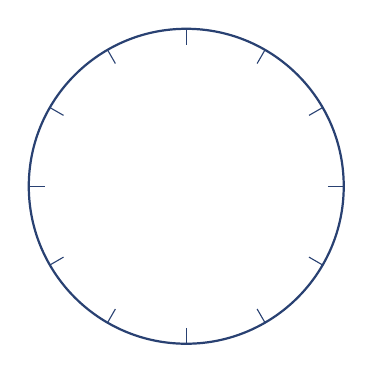
\begin{tikzpicture}
        \draw[headerblue, thick] (0,0) circle (2cm);
        \foreach \i in {1,...,12} {
            \draw[headerblue] ({30*\i}:1.8) -- ({30*\i}:2);
        }
    \end{tikzpicture}
    
    \vspace{1cm}
    
    {\LARGE \VAR{name}}
    
    \vspace{0.5cm}
    
    {\large Born: \VAR{birth_date} at \VAR{birth_time}}
    
    \vspace{0.3cm}
    
    {\normalsize Location: \VAR{latitude}$^\circ$ N, \VAR{longitude}$^\circ$ E}
    
    {\normalsize Timezone: UTC\VAR{timezone}}
    
    \vfill
    
    {\small Generated using Swiss Ephemeris}
    
    {\small \VAR{generated_date}}
\end{titlepage}

% Summary Page
\section{Birth Chart Summary}

\begin{center}
\begin{tabular}{ll}
    \textbf{Moon Sign (Rashi):} & \VAR{moon_rashi} \\
    \textbf{Moon Nakshatra:} & \VAR{moon_nakshatra} (Pada \VAR{moon_pada}) \\
    \textbf{Ascendant (Lagna):} & \VAR{ascendant_rashi} \\
    \textbf{Nakshatra Lord:} & \VAR{nakshatra_lord} \\
    \textbf{Ayanamsa:} & Lahiri (\VAR{ayanamsa}$^\circ$) \\
\end{tabular}
\end{center}

\section{Moon Nakshatra: \VAR{moon_nakshatra}}

\begin{tabular}{@{}ll@{}}
    \textbf{Deity:} & \VAR{nakshatra_deity} \\
    \textbf{Ruling Planet:} & \VAR{nakshatra_lord} \\
    \textbf{Symbol:} & \VAR{nakshatra_symbol} \\
    \textbf{Nature:} & \VAR{nakshatra_nature} \\
    \textbf{Pada:} & \VAR{moon_pada} \\
\end{tabular}

\subsection{Interpretation}

\VAR{nakshatra_interpretation}

\section{Moon Sign: \VAR{moon_rashi}}

\begin{tabular}{@{}ll@{}}
    \textbf{Element:} & \VAR{rashi_element} \\
    \textbf{Quality:} & \VAR{rashi_quality} \\
    \textbf{Ruler:} & \VAR{rashi_ruler} \\
    \textbf{Position:} & \VAR{moon_degree_in_sign} in sign \\
\end{tabular}

\subsection{Interpretation}

\VAR{rashi_interpretation}

\newpage

\section{Planetary Positions}

\begin{table}[h]
    \centering
    \begin{tabular}{lccccc}
        \toprule
        \textbf{Planet} & \textbf{Sign} & \textbf{Longitude} & \textbf{Nakshatra} & \textbf{Pada} & \textbf{R} \\
        \midrule
        % PLANETS_TABLE
        \bottomrule
    \end{tabular}
\end{table}

\small R = Retrograde

\section{Vimshottari Dasha Periods}

The Vimshottari Dasha system is based on your Moon's Nakshatra (\VAR{moon_nakshatra}). Your birth Dasha is \VAR{starting_dasha}.

\begin{table}[h]
    \centering
    \begin{tabular}{lccc}
        \toprule
        \textbf{Mahadasha} & \textbf{Years} & \textbf{Start} & \textbf{End} \\
        \midrule
        % DASHA_TABLE
        \bottomrule
    \end{tabular}
\end{table}

\section{Notes}

\begin{itemize}
    \item All calculations use the Lahiri Ayanamsa, the most commonly used in Indian astrology
    \item Planetary positions are given in the sidereal zodiac
    \item The Vimshottari Dasha is a 120-year planetary period system
    \item Rahu and Ketu are the Moon's North and South nodes respectively
\end{itemize}

\vfill

\begin{center}
    \small\textit{Generated using Swiss Ephemeris with Lahiri Ayanamsa}
    
    \small Report Date: \VAR{generated_date}
\end{center}

\end{document}
